%\chapter{Implementation}
%\label{chap:impl}

%The implementation chapter describes various software components both developed and fitted to create a framework for programming in Rust for an Embedded system.
%The last sections dives into two projects which were developed in order to drive the deveopment of the framework and to provide a basis to evaluate the platform in the next chapter.

%We start in \autoref{sec:impl:booting} by describing the startup process of a Rust program on a Microcontroller.
%Secondly we define the parts of the Rust standard library \gls{rel} which are applicable for an embedded system.
%In \autoref{sec:impl:oo} we look at the how and why the Object Oriented paradigm can be applied to hardware devices.
%\autoref{sub:interfacing_with_emlib} goes on to describe the hardware specific bindings developed for controlling the Peripherals of the Microcontroller.
%In \autoref{sec:build_system} we take a look at the evolution of the building system from a traditional \file{Makefile} to the integration with the {\rust} package manager {\cargo}.
%The next two sections \autoref{sec:irq-closures} and \autoref{sec:rust-embedded-modules} explores a few experimentation with creating higher level abstractions for the lower level Peripheral libraries.
%\autoref{sec:porting-gpioint} looks at a case study of porting a GPIO driver from {\C} to {\rust}.
%The last section \autoref{sec:impl:projects} gives an overview over the implementation of the projects used to evaluate the programmability and certain metrics presented in \autoref{chap:results}.

\newcommand{\corechapter}[3]{
  \chapter{#1}
  \label{chap:#2}
  \begin{center}
    \includegraphics{figures/RustyGecko-#2}
  \end{center}
  \hfill \break
  \hfill \break
  \hfill \break
#3
}

\corechapter{Startup}{startup}{%
  The startup module handles the process of starting an {\rust} application on the \gls{mcu}.
  This involves supporting some basic requirements for the language and setting up some important initialization of the processor.
  This module is a foundation, but can be used in isolation to run a program on the \gls{mcu} without any more dependencies.
}
\section{Booting {\rust} on the {\gecko}}

The contains of this section explaines how the startup process described in \autoref{sec:back:startup} is implemented for a {\rust} program.

The process for {\rust} is identical to the process in C due to the fact that {\rust} only allows constant initialization before the {\main} function.
In C++ however, the process is complicated by the fact that C++ support static global constructors as shown in \autoref{lst:impl:c++:static-constructor}

\begin{listing}[H]
  \begin{minted}{c++}
class Foo { Foo() { } };
Foo foo;
int main() { return 0; }
  \end{minted}
  \caption{}
  \label{lst:impl:c++:static-constructor}
\end{listing}

In \autoref{lst:impl:c++:static-constructor} the Foo constructor call must be issued before the main function is executed.
The runtime must therefore be augmented to issue calls to these constructors and handle errors that can occure.
These types of constructors are not allowed in {\rust} by a compiler rule which allows only constant-expression as initializers.
(An interesting side note here is given in \autoref{sec:impl:lazy-statics}.)

As this process is identical to C we are able to reuse standard runtime components for embedded toolchains for C.
SiliconLabs software suite provides the \func{ResetHandler} and linker script for the efm32 microcontrollers.
The \func{\_mainCRTStartup} function defined in the C runtime provided by the \textbf{arm-none-eabi} gcc toolchain handles the setup in \func{\_start}:

\subsection{Minimal {\rust} program to boot}

There are a few modification which have to be applied to the default 'Hello World' program in order to get it to boot in an embedded environment.
Lets first look at the standard version in \autoref{lst:rust-hello-world}.

\begin{listing}[H]
\begin{minted}{rust}
fn main() {
  println!("Hello, World!");
}
\end{minted}
\label{lst:rust-hello-world}
\caption{\rust Hello World}
\end{listing}

In comparrison, the embedded version in \autoref{lst:embedded-rust-hello-world}.
This program does not print out "Hello, World!" as this requires some setup and we are conserned with the boot processs here.
The highlight of the changes are, to export the {\main} function to the C runtime, and to prevent the standard library being loaded while retaining the core library.

\begin{listing}[H]
\begin{minted}{rust}
#![no_std]
#![no_main]
#![feature(lang_items)]

extern crate core;

#[no_mangle]
pub extern "C" fn main() {
  loop {}
}

#[lang="stack_exhausted"] extern fn stack_executed() {}
#[lang="eh_personality"] extern fn eh_personality() {}
#[lang="panic_fmt"] fn panic_fmt() -> ! { loop {} }
\end{minted}
\caption{Embedded Hello World}
\label{lst:embedded-rust-hello-world}
\end{listing}

\attrib{\#\![no\_std]} on line 1 in \autoref{lst:embedded-rust-hello-world} tells the {\rust} compiler not to include the standard library.
The standard library is not used for embedded programming. \todo{include reasoning or refere to section about not using std}

Line 2 must be analysed in conjunction with lines 7 and 8.
Firstly we must guarantee that the function can be called by the \func{\_start} function.
This is done by defining the {\main} function to be an publicly exported symbol denoted by \code{pub extern}.
\rust symbols are private by default.
The second change is to ensure that the function is callable by the a C function.
\code{extern "C"} makes this possible by making the function use the C ABI. \todo{Some reference to the C ABI}
The last thing is to disable the {\rust} name mangling so that the C code can refere to the function by the unmangled name {\main}.
Now that the {\main} function is altered to be callable by C, the function does not resemble the function the rust compiler expects to find.
Therefore we have to tell the compiler that the program does not contain a {\main} function, but that this is ok, hence the \attrib{\#\![no\_main]}.

The last three lines are a complication due to error handling in {\rust}.
These functions are used by the core library but implemented in the standard library, they are described in detail in Section \ref{}. \todo{Describe panic and exception handling}
The implementation here just ignores all error handling.

\todo{Might go in a different section}
With an example, we will now see how the startup process maps to the storage qualifiers in {\rust}.
\begin{listing}[H]
\begin{minted}{rust}
const      RUST_CONST_ZERO: u32 = 0;      // not allocated
const      RUST_CONST: u32 = 0xFEED;      // not allocated
static     RUST_STATIC_ZERO: u32 = 0;     // .text
static     RUST_STATIC: u32 = 0xDEAD;     // .text
static mut RUST_STATIC_MUT_ZERO: u32 = 0; // .bss
static mut RUST_STATIC_MUT: u32 = 0xBEEF; // .data

pub extern fn main() { /* Use the variables */ }
\end{minted}
\caption{\rust static initialization}
\label{lst:rust-static-init}
\end{listing}
In \autoref{lst:rust-static-init} the three different types of declaring globals in {\rust} are shown.
Firstly {\rust} divides between two types of global declarations, constants and statics.
The static globals are immutable by default but can be made mutable by the \code{mut} keyword.
A constant declaration, shown in lines 1 and 2 of \autoref{lst:rust-static-init}, represents a value.
There is no need to allocate memory for globals declared as \code{const} and they behave like \code{\#define} in C. \todo{Well that's a lie as \#define is handled by the preprocessor}
Variables on line 3 and 4 declares the variables to be \code{static}.
As these are immutable they are allocated in the read-only section called {\elf}sec{.text}.
On line 5 and 6 the declarations are marked with \code{static mut}.
Here we see that the zero initializes variable is assigned to the {\elf}sec{.bss} section in the {\elf} file.
On line 6 we have a non-zero value that has to be stored in Flash memory prior to execution and is copied to RAM in the \func{ResetHandler}.


\corechapter{Rust Embedded Library}{rel}{%
  The \gls{rel} module defines the subset of the standard {\rust} library which is applicable for embedded applications.
  This module builds on the foundation layed out by the startup module and is used by the Bindings and Application Layer modules of the {\rg} platform.
}
% !TEX root = ../main.tex

\section{The Core Library}
\label{sec:rust:core}

As described in \autoref{sec:rcl}, the \gls{rcl} defines the \emph{core} functionality of the {\rust} language.
The \gls{rcl} does not have any library dependencies, but in order to use the library without \gls{rsl} a few definitions are needed.
These definitions are given in \autoref{tab:core:definitions}.

\begin{table}[H]
  \centering
  \begin{tabular}{l | l}
    \textbf{Functions} & \textbf{Description} \\
    \hline
    \code{memcpy, memcmp, memset} & Basic memory management \\
    \code{rust\_begin\_unwind}    & Handles panicking \\
    \hline
  \end{tabular}
  \caption{External dependencies of \gls{rcl}}
  \label{tab:core:definitions}
\end{table}

The memory management functions given in \autoref{tab:core:definitions} are provided by \lib{newlib} and are exposed through the \lib{startup} library described in \autoref{sec:startup}.
These functions provide the basic memory management that is needed in order to utilize the parts of \gls{rsl} that defines dynamically allocated data structures.

\concept{Panicking} is {\rust}'s way of unwinding the currently executing thread, ultimately resulting in the thread being terminated.
A panic in {\rust} can happen, e.g. when an array is indexed out of bounds, which causes the \code{rust\_begin\_unwind} function to be called.
The \code{rust\_begin\_unwind} is also defined in \lib{startup}, but the implementation is only an infinite loop to aid debugging.
In contrast, the definition of \code{rust\_begin\_unwind} given in \gls{rsl} will abort the program and print an error message.

\section{The Allocation Library}
\label{sec:rust:allocation}

Heap allocation is introduced in a library called \lib{alloc}.
The library defines the managed pointer, \code{Box}, which is {\rust}'s main means of allocating memory on the heap.
Also, the allocation library defines the types \code{Rc} and \code{Arc}, which are {\rust}'s \emph{reference counted} and \emph{atomically reference counted} heap pointers.

\begin{listing}[H]
  \begin{rustcode}
fn rust_allocate(usize, usize) -> *mut u8;
fn rust_deallocate(*mut u8, usize, usize);
fn rust_reallocate(*mut u8, usize, usize, usize) -> *mut u8;
  \end{rustcode}
  \caption{External dependencies of the \lib{alloc} library}
  \label{tab:alloc:external-funcs}
\end{listing}

The allocation library is by default dependent on \lib{libc}, but this dependency can be broken by supplying the \flag{--cfg feature="external\_funcs"} flag to the compilation process.
When breaking this dependency, the allocation library requires the functions in \autoref{tab:alloc:external-funcs} to be defined elsewhere.
Note that these functions map directly to the \code{alloc}, \code{dealloc}, and \code{realloc} functions, which all are part of {\newlib}.
This design makes it easy to include the {\lib{alloc}} library for new platforms like {\rg}.

\section{The Collection Library}

The {\rust} \lib{collections} library provides general purpose data structures.
Out of these data structures the \code{Vector} (a growable heap allocated list) and the \code{String} (heap-allocated mutable strings) are the most notable.

As one would expect, the \lib{collections} library depends on the \lib{alloc} library, as it needs to allocate memory on the heap.
\texttt{collections} also depends on the \texttt{unicode} library because all strings in {\rust} are UTF-8 encoded.

\section{The Rust Embedded Library}
\label{sec:rel}

The libraries mentioned in the previous sections provides core language constructs and dynamic heap allocation.
Together they form a strong foundation for new {\rust} programs, without depending on an \gls{os}.
We have composed these libraries into what we refer to as the \gls{rel}, and the dependencies of these libraries are is shown \autoref{fig:rust:rel}.

\begin{figure}[H]
  \begin{center}
    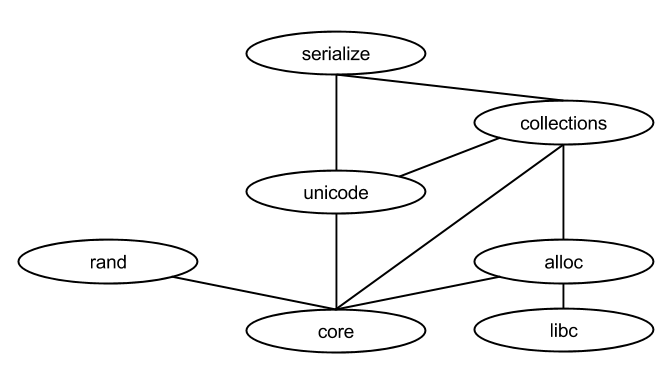
\includegraphics[scale=0.3]{figures/background/rust/embedded-rust-lib.png}
  \end{center}
  \caption{Rust Embedded Library}
  \label{fig:rust:rel}
\end{figure}

It is important to note that \gls{rel} is just a way to provide a well-defined definition of the {\rust} language for an embedded system.
\gls{rel} is, unlike \gls{rsl}, not built as a facade, it is nothing but a collection of freestanding {\rust} libraries that are suited for an embedded system.
However, the libraries that make up \gls{rel} needs to be conditionally compiled for the Cortex-M3 architecture, and this is described in \autoref{chap:build}.



\corechapter{Binding Libraries}{bindings}{%
  The Bindings module includes the peripheral libraries provided by the \gls{mcu} vendor SiliconLabs, and the architecture designer ARM.
  In order to make use of these libraries in {\rust} we developed binding libraries to expose the underlying {\C} implementation to the {\rust} language.
}
\section{Object-oriented Embedded Programming}
\label{sec:impl:oo}

The interface of many of the modules defined in {\emlib} resembles that of objects found in object-oriented programming.
In its essence, object-oriented programming focuses on organizing a computer program by looking at the data the program operates on.
This is done by grouping related data into objects and defining methods that operate on the data contained within the objects.

The paradigm's essential concept can be applied to embedded {\C} programming, even though the language itself does not directly define any language features to aid the design.
In this section, we look at how control over the memory layout of objects, and static dispatch, can be used to enable the object-oriented paradigm in conjunction with \gls{mmio} in embedded programming.
We use the memory layout of a memory-mapped \gls{adc} as an example to see how this peripheral can be represented as an object.

Static dispatch, as opposed to dynamic dispatch, is the mechanism in which the function to be called can be decided statically by the compiler, and a \code{call} instruction to the function can be inserted into the code directly.
Dynamic dispatch, on the other hand, requires extra runtime information about the function to be called, which adds an additional layer of indirection to the function call.
% Dynamic dispatch, on the other hand, requires runtime information which requires the call to the function to be made through an extra layer of indirection.


\subsection{Memory Mapped I/O}
\label{ssec:memory_mapped_io}

\gls{mmio} is a method for interfacing with peripheral devices in a computer system.
The method entails connecting the control registers of hardware devices to the same address bus as \gls{ram}.
This results in a programming model where the programmer can use common memory operations to control the devices.

Let us consider the \gls{adc} on the {\gecko}.
The \gls{adc} converts an analog signal to a digital representation.
The base address of the \gls{adc} on the {\gecko} is memory mapped to the location \mem{0x40002000} in the memory space.
This means that writing to a pointer that points to this address will write to the control registers in the \gls{adc} device.

\begin{figure}[H]
  \centering
  \begin{tabular}{l|l|l|}
    \textbf{Location} & \textbf{Offset} & \textbf{Name} \\
    \hline
    &...&...\\
    \hline
    \hline
    \mem{0x40002000} & 0x0 & CTRL\\
    \hline
    & \mem{0x4} & CMD\\
    \hline
    &...&...\\
    \hline
    & \mem{0xC} & SINGLECTRL\\
    \hline
    &...&...\\
    \hline
    & \mem{0x24} & SINGLEDATA\\
    \hline
    &...&...\\
    \hline
    \hline
    &&\\
  \end{tabular}
  \caption{Subsection of ADC0 Memory map for the {\gecko}}
  \label{fig:back:memorymapped}
\end{figure}

\autoref{fig:back:memorymapped} shows a subsection of \gls{ram} that contains the \gls{adc} control register.
Only the relevant registers for our discussion in included in the figure.
It shows the control register that is used when performing a single \gls{adc} conversion.
Note that it only includes the register needed for this kind of conversion.
The CTRL register is used to initialize the hardware device before performing a conversion, and the CMD register is used to issue direct commands to the device like \emph{stop} and \emph{start}.
We see that the CTRL register is at offset \mem{0x0} from the base address of the \gls{adc} and that the CMD register is at an offset of \mem{0x4} bytes.
The two registers, SINGLECTRL and SINGLEDATA, are there for initializing the single conversion and read the results of a conversion, respectively.

\subsection{Memory Layout of Objects}

The traditional memory layout of an object in an object-oriented language is an implementation detail.
This is because the fields of the object might have different sizes, and optimizations can rearrange the memory layout to optimize for size.
The layout is also an implementation detail of {\rust} for the same reasons, but by annotating a struct with \attrib{\#[repr(C)]}, it will ensure that it is compatible with {\C}'s \gls{ffi}.
Objects in a language like {\Java} also includes a tag field at the base of the object as a reference to the class of the object in order to provide dynamic dispatch.

\begin{listing}[H]
  \centering
  \begin{minipage}{0.26\textwidth}
  \begin{listing}
    \begin{javacode}
class ADC {
  int CTRL;
  int CMD;
  // ...
  int SINGLECTRL;
  // ...
  int SINGLEDATA;
  // ...
}
    \end{javacode}
  \end{listing}
  \end{minipage}
  \hfill
  \begin{minipage}{0.27\textwidth}
  \begin{listing}
    \begin{rustcode}
#[repr(C)]
struct ADC {
  CTRL: u32,
  CMD: u32,
  // ...
  SINGLECTRL: u32,
  // ...
  SINGLEDATA: u32,
  // ...
}
    \end{rustcode}
  \end{listing}
  \end{minipage}
  \hfill
  \begin{minipage}{0.33\textwidth}
  \begin{listing}
    \begin{ccode}
typedef struct {
  uint32_t CTRL;
  uint32_t CMD;
  // ...
  uint32_t SINGLECTRL;
  // ...
  uint32_t SINGLEDATA;
  // ...
} ADC;
    \end{ccode}
  \end{listing}
  \end{minipage}

  \caption{Definition of an \gls{adc} in {\Java}, {\rust}, and {\C}}
  \label{lst:back:adc-objects}
\end{listing}

In {\C}, where classes and objects are not part of the language, structs are used to create the representations for objects.
By using structs, the programmer has full control over the layout of the object in memory.
The object-oriented concepts used for \gls{mmio} uses static dispatch, and the structs do not include tag fields or references to virtual tables.
\autoref{lst:back:adc-objects} shows how to define a {\Java} class, and {\rust} and {\C} structs for the \gls{adc} on the {\gecko}.
The memory layout of these objects is given in \autoref{fig:back:memlayout}.

\begin{figure}[H]

  \centering
  \begin{subfigure}{0.31\textwidth}
    \begin{tabular}{|l|l|}
      \hline
      0x0&Object tag \\ \hline
      0x4&CTRL       \\ \hline
      0x8&CMD        \\ \hline
      ...&...        \\ \hline
      0x10&SINGLECTRL\\ \hline
      ...&...        \\ \hline
      0x28&SINGLEDATA\\ \hline
      ...&...        \\ \hline
    \end{tabular}
    \caption{{\Java}}
    \label{fig:back:memlayout:java}
  \end{subfigure}
  \hfill
  \begin{subfigure}{0.31\textwidth}
    \begin{tabular}{|l|l|}
      \hline
      0x0&CTRL       \\ \hline
      0x4&CMD        \\ \hline
      ...&...        \\ \hline
      0xC&SINGLECTRL \\ \hline
      ...&...        \\ \hline
      0x24&SINGLEDATA\\ \hline
      ...&...        \\ \hline
    \end{tabular}
    \caption{\rust}
    \label{fig:back:memlayout:rust}
  \end{subfigure}
  \hfill
  \begin{subfigure}{0.31\textwidth}
    \begin{tabular}{|l|l|}
      \hline
      0x0&CTRL       \\ \hline
      0x4&CMD        \\ \hline
      ...&...        \\ \hline
      0xC&SINGLECTRL \\ \hline
      ...&...        \\ \hline
      0x24&SINGLEDATA\\ \hline
      ...&...        \\ \hline
    \end{tabular}
        \caption{{\C}}
    \label{fig:back:memlayout:c}
  \end{subfigure}
  \caption{Memory layout of objects}
  \label{fig:back:memlayout}

\end{figure}

By comparing \autoref{fig:back:memorymapped} and \autoref{fig:back:memlayout}, we see that the memory layout of a struct defined in {\rust} and {\C} has the exact same layout as the memory mapped control register of the \gls{adc}.
This suggests that, if a pointer to the \gls{mmio} device is considered as a reference to an \gls{adc} object, the object-oriented pattern can be used to directly interface with the \gls{mmio}.

The layout of the {\Java} object in \autoref{fig:back:memlayout:java} could imply that the same analysis can be applied by adding an offset, equal to the size of the object tag, to the reference.
This is not the case as this would map the object tag to the base address of the \gls{adc} minus 4 bytes.
This location is, in the case for the {\gecko}, an unmapped memory section used to add padding between the \gls{adc} and the previous \gls{mmio}.
{\Java} uses this object tag to store a reference used to dynamically dispatch method calls to the object.
Moreover, using the reference in place of a regular {\Java} object would cause the method dispatch mechanism to fail.

\subsection{Adding Object Functionality}

This section shows how we add functionality called \emph{methods} to the \gls{mmio} objects.
Both {\C} and {\rust} uses static dispatch.
This ensures that {\C} and {\rust} provide the same zero-cost abstractions when interacting with the \gls{mmio}.

\subsubsection{Static Dispatch in C}

Implementing objects with static dispatch is a straight forward process in {\C}.
Here, we define a function which takes a reference to the object as the first parameter.
The function then uses the object reference in the same manner as the implicit \var{this} parameter in conventional object-oriented languages such as {\Java}.

\begin{listing}[H]
  \centering
  \begin{minipage}{0.47\textwidth}
  \begin{listing}
      \begin{ccode}
// ADC Member function with
// explicit object reference
uint32_t ADC_DataSingleGet(
           ADC *const adc) {
  // The adc pointer is used as a
  // reference to the this object
  return adc.SINGLEDATA;
}

void main() {
  // The next section describes
  // how to instantiate MMIOs
  ADC adc;
  // Call the member function
  // passing in an explicit
  // reference to the object
  ADC_DataSingleGet(&adc);
}
      \end{ccode}
  \end{listing}
  \end{minipage}
  \hfill
  \begin{minipage}{0.47\textwidth}
  \begin{listing}
      \begin{rustcode}
impl Adc {
  // Rust lets the programmer
  // specify how to accept the
  // object when invoked with
  // the dot notation
  pub fn data_single_get(&self)
  -> u32 { // self is a reference
    // to the ADC MMIO
    self.SINGLEDATA
  }
}

fn main() {
  // Instantiation of MMIOs is
  // handled in the next section
  let adc = Adc;
  // The Rust compiler issues
  // a static call to the
  // member method and passes in
  // the reference to the MMIO
  adc.data_single_get();
}
      \end{rustcode}
  \end{listing}
  \end{minipage}
  \caption{Member methods for {\C} and {\rust}, respectively.}
  \label{lst:back:adc:get}

\end{listing}

\autoref{lst:back:adc:get} shows how to define a getter function for the \gls{adc} single conversion register as a member method using an object-oriented pattern.
We use the \keyword{impl} block to define the same behavior in {\rust}, but the methods are called with the dot notation known from object-oriented languages.

\subsection{Instantiating a MMIO object}

Now that we have shown that \glspl{mmio} can be represented as objects defined by structs, we consider how to instantiate them.
Usually, an object in the object-oriented paradigm is created with a constructor and deallocated with a destructor.
The constructor is responsible for allocating the object and initializing the fields with values.
Analogously, the destructor is responsible for deallocating the object and any other member objects that it owns.
\gls{mmio} devices have a fixed position in the memory and do not need to be allocated, and they also generally do not have any owned members.
Therefore the constructor-destructor pattern is not applicable for \gls{mmio}s, but we still need to instantiate the variable that holds the reference to the \gls{mmio} and cast it to the desired type.
\autoref{fig:oo:instantiate} shows how to instantiate a \gls{mmio} as an object in both {\C} and {\rust}.

\begin{listing}[H]
  \begin{minipage}{0.46\textwidth}
  \begin{listing}
    \begin{rustcode}
const ADC0_BASE: *mut Adc
      = 0x40002000 as *mut Adc;

fn main() {
  let adc0 = unsafe {
    ADC0_BASE.as_mut().unwrap()
  };
}
    \end{rustcode}
    \caption{Rust}
  \end{listing}
  \end{minipage}
  \hfill
  \begin{minipage}{0.45\textwidth}
  \begin{listing}
    \begin{ccode}
#define ADC0_BASE 0x40002000

void main() {
  ADC* adc0 = (ADC*)ADC0_BASE;
}
    \end{ccode}
    \caption{{\C}}
  \end{listing}
  \end{minipage}
  \caption{Instantiating a \glspl{mmio}}
  \label{fig:oo:instantiate}
\end{listing}

%For a further discussion of this pattern in {\rust}, see \autoref{sec:res:aliasing-mmios}.

% !TEX root = ../main.tex

\section{Library Bindings}
\label{sub:interfacing_with_emlib}

This section describes the peripheral library \emph{bindings} developed for the platform.

The \gls{ffi} available in {\rust} has been used to interface with Silabs' suite of C libraries used to control the {\gecko}.
This way, we have been able to create wrappers around the \gls{api} for the different peripherals that we have used in the project, without porting the core logic itself.
These wrappers are called language bindings.
The following sections explain the process of defining and implementing the \gls{ffi} in {\rust} that is used to access and control the peripherals on the {\gecko}.

\subsection{The Libraries}
\label{ssub:the_bindings_library}

In \autoref{sec:back:lib} we presented the three libraries we have created partially binding support for, CMSIS, Emlib and Emdrv.
Here we will take a closer look at which modules have been developed and an reasoning for chosing each one.

We have written many example applications in {\rust} that utilize the bindings for many of the {\gecko}'s peripherals, these examples have been a driving factor for defining new bindings.
As an example, if we were to need some functionality for the \gls{adc}, we would define these bindings alongside the development of the examples.
In this way, the bindings have been defined incrementally during the development of either the examples that demonstrate our libraries, or the applications described in \autoref{sec:impl:project:i} and \autoref{sec:impl:project:ii}.

\subsubsection{CMSIS}
\label{sub:cmsis_bindings}

Interrupt support through \gls{nvic} was the only interesting part of the \gls{cmsis} library that we have written bindings for.
Most of the examples uses one or several IRQ handlers for the peripheral bindings that they demonstrate.
\gls{nvic} provides utility functions for enabling and disabling the interrupt handling mechanisms of the Cortex-M3 processor.

\subsubsection{Emlib}

The priority, when we first set out to make the bindings for {\emlib}, was to define a viable platform to write rust applications with, which we could use to evaluate the language on the embedded system.
It has not been a priority of this project to fully support all of the {\gecko}'s peripherals or provide bindings for the entire {\emlib}.
The bindings have been developed because we have needed functionality from the peripherals, not the other way around.
\autoref{tab:emlib_peripheral_bindings} summarizes a number of modules from {\emlib} that we have written bindings for, and why we wanted these bindings.
A list of examples that demonstrates how the bindings work is shown in \autoref{tab:emlib_examples}, these are either written from scratch, or directly ported from {\emlib}'s examples.

\begin{table}[H]
  \centering
  \begin{tabular}{r|p{10cm}}
    \textbf{Module} & \textbf{Purpose} \\
    \hline
\prog{cmu}     &
The \gls{cmu} provides functions to manage the different clocks and oscillators on the {\gecko}.
This module is necessary in order to configure the clocks that are required by other peripherals to function. \\

\prog{dma}     &
We wanted to use \gls{dma} for the {\prog{sensor-tracker}} application because it can be used to transfer data without using the \gls{cpu}. \\

\prog{ebi}     &
The \gls{ebi} is used in the {\gecko}'s internal memory map, and simplifies the process of writing data to e.g. the LCD on the {\chip{DK}}. \\

\prog{emu}     &
The \gls{emu} module controls the different energy modes on the {\gecko}.
We needed this functionality for the {\prog{sensor-tracker}} application. \\

\prog{gpio}    &
The \gls{gpio} was one of the first modules to be ported, it is used extensively throughout the bindings and in the applications. \\

\prog{lesense} &
The \gls{lesense} can be configured to automatically collect data from multiple sensors, we needed this for the {\prog{sensor-tracker}}. \\

\prog{acmp}    &
The \gls{acmp} was ported alongside \gls{lesense}, it is used to compare two analog signals and tell which one is greater. \\

\prog{adc}     &
The \gls{adc} was needed by the {\prog{sensor-tracker}}, it has been used to get the internal temperature of the \gls{cpu}. \\

\prog{usart}   &
Primarily we wanted the \gls{usart} for easy debugging and I/O from a computer. \\

\prog{leuart}  &
The \gls{leuart} was ported a while after the \gls{usart}.
It has the same functionality, but it works with a lower-frequency clock and at requires less energy than the \gls{usart}. \\

\prog{i2c}     &
The \gls{i2c} protocol has many of the same use cases as the different \gls{uart} types, bbut it works at lower energy levels.
It is used by the {\prog{sensor-tracker}}. \\

\prog{rtc}     &
The \gls{rtc} was an easy module to write bindings for, it is used in several examples for timing purposes, as well as in the {\prog{sensor-tracker}}. \\

\prog{timer}   &
The Timer was one of the first modules to be ported, it worked as a proof-of-concept for the design of the bindings, as described earlier in this section. \\

    \hline
  \end{tabular}

  \caption{Peripheral bindings for {\emlib}.}
  \label{tab:emlib_peripheral_bindings}
\end{table}


\begin{table}[H]
  \centering
  \begin{tabular}{r|p{8cm}|c}
    \textbf{Example} & \textbf{Purpose} & \textbf{Ported} \\
    \hline
\prog{buttons\_int}  &
Demonstrates interrupts by lighting a led on the {\chip{STK}} when the respective button has been pressed. & \cmark \\

\prog{rtc\_blink}    &
Toggle a led with an interval of 2 seconds. & \cmark \\

\prog{energy\_modes} &
Demonstrates the four stages of sleep on the {\gecko}. & \cmark \\

\prog{uart}          &
Demonstrates serial communication over \gls{uart} by echoing back every byte it receives. & \cmark \\

\prog{leuart}        &
Similar example as \prog{uart}, but the \gls{cpu} is turned off and the functionality is moved to an interrupt handler instead. & \cmark \\

\prog{i2c}           &
Sends and receives a data-buffer between two devices that supports \gls{i2c}. & \cmark \\

\prog{joystick}      &
Reads analog signals generated by a Joystick that is connected to the {\chip{STK}}. & \\

{\prog{dma}}           &
Transfer a data-buffer from one memory location to another. & \cmark \\

\prog{light\_sense}  &
Uses the {\chip{STK}}'s light sensor to measure the light intensity, and ligts a LED when the intensity goes below a threshold & \cmark \\

\prog{boxes}         &
Demonstrates dynamic memory allocation with \code{Box}'es, provided by the {\rust} \lib{alloc} library.  &  \\

\prog{vec}           &
Demonstrates dynamically allocated strings and vectors from the \lib{collections} library. & \\

    \hline
  \end{tabular}

  \caption{Examples that demonstrates how the bindings work.}
  \label{tab:emlib_examples}
\end{table}

\subsubsection{Emdrv}
\label{sub:emdrv_bindings}

As with {\emlib}, it was not a goal to fully support all available peripheral drivers that are available in \prog{emdrv}.
The drivers that we have partially implemented bindings for are summarized in \autoref{tab:emdrv_bindings}, they are not that hard to grasp or use since they are all fairly small.
The project includes two examples that demonstrate how to use the flash driver, they are summarized in \autoref{tab:emdrv_examples}  \todo{table needs to refer to section about IRQ. Evt. flytt noe av innholdet fra IRQ-seksjonen inn i denne seksjonen.}.

\begin{table}[H]
  \centering
  \begin{tabular}{r|p{10cm}}
    \textbf{Driver} & \textbf{Purpose} \\
    \hline

\prog{dmactrl}  &
This binding only exports one function to return a standard \emph{\gls{dma} Descriptor} which is used to initiate a \gls{dma} transfer. \\

\prog{flash}  &
The flash driver adds an abstraction layer over a flash memory, it exposes functions to \emph{initialize}, \emph{read}, \emph{write} and get the \emph{device info}.
The Driver is used by the {\prog{sensor-tracker}}. \\

\prog{gpioint}  &
This driver is ported from {\C} to {\rust}, the implementation differs slightly between the two versions, but the functionality is the same.
The reasoning for porting this driver is described in \autoref{}. \\

\prog{i2c}  &
This driver is used by the {\prog{sensor-tracker}} application, it exposes functions to initalize a commonly used \gls{i2c} data transfer configuration. \\

\prog{tft}  &
This binding exposes one function to initialize the TFT screen on the {\chip{DK}}.
It is used in the \prog{circle-game}. \\

    \hline
  \end{tabular}

  \caption{Driver bindings for \prog{emdrv}.}
  \label{tab:emdrv_bindings}
\end{table}

\begin{table}[H]
  \centering
  \begin{tabular}{r|p{8cm}|c}
    \textbf{Example} & \textbf{Purpose} & \textbf{Ported} \\
    \hline

\prog{flash} &
Demonstrates reading and writing to the {\chip{STK}}'s flash memory. & \cmark \\

\prog{light\_measure} &
Based on the \prog{light\_sense} example from \autoref{tab:emlib_examples}.
The results from measuring the light intensity is saved to flash.
When the user presses a button the {\chip{STK}} will initiate a transfer that reeds all the data stored to flash and transmits it over a \gls{usart} connection. & \cmark \\

    \hline
  \end{tabular}

  \caption{Examples that demonstrate how to use the flash bindings.}
  \label{tab:emdrv_examples}
\end{table}

\subsection{Defining the Bindings}

The {\emlib} module for controlling the \code{Timer} peripheral \cite{an0014_timer} works as a good example to demonstrate what the {\rust} bindings look like.
The module is fairly small, it mostly exposes functions to set up and initialize four different timers that can be used for up, down, up/down, and input- and output-capture.
The program shown in \autoref{lst:timer_program_c} is an example of initializing the \code{Timer0} peripheral on the {\gecko}, note that this is not a complete working example, it only shows the most important parts required to use the Timer module.
Then an initialization structure for the Timer module is acquired, this structure has fields to configure many different properties of the Timer, in the same way as described in \autoref{ssec:memory_mapped_io}.

\begin{listing}[h]
\begin{minted}{c}
// Select TIMER0 parameters
TIMER_Init_TypeDef timerInit = TIMER_INIT_DEFAULT;
// Enable overflow interrupt
TIMER_IntEnable(TIMER0, TIMER_IF_OF);
// Enable TIMER0 interrupt vector in NVIC
NVIC_EnableIRQ(TIMER0_IRQn);
// Set TIMER Top value
TIMER_TopSet(TIMER0, TOP);
// Configure TIMER
TIMER_Init(TIMER0, &timerInit);
\end{minted}
\caption{Initializing a Timer in C}
\label{lst:timer_program_c}
\end{listing}

The next lines enable interrupts for the Timer, and the \gls{nvic} interrupt vector is set up to call the function shown in \autoref{lst:timer_interrupt_handler} every time an interrupt it triggered by the Timer.
All this function does is to clear the interrupt signal and toggle the value of an LED.
We can imagine an application where the Timer is configured to trigger an interrupt every minute to toggle the LED, and in between the interrupts the \gls{mcu} can be put to sleep in order to save power.
Interrupts like this are an important part of programming the {\gecko}.
They can be used for an asynchronous programming model where the application is defined by the code in the different interrupt handlers, and like in the example above, the \gls{mcu} can be put to sleep in between interrupts.

\begin{listing}[h]
\begin{minted}{c}
void TIMER0_IRQHandler(void) {
  // Clear flag for TIMER0 overflow interrupt
  TIMER_IntClear(TIMER0, TIMER_IF_OF);
  // Toggle LED ON/OFF
  GPIO_PinOutToggle(LED_PORT, LED_PIN);
}
\end{minted}
\caption{Timer Interrupt Handler}
\label{lst:timer_interrupt_handler}
\end{listing}

The equivalent program written in {\rust} is shown in \autoref{lst:timer_program_rust}.
Semantically they are the same, but the usage differs slightly, which is natural since we are using a higher level programming language.
Instead of calling functions that are included through a {\C} header file, we are calling functions that are available through a {\rust} module.
For example the \func{enable\_irq} function is part of the \code{nvic} module.
This modularization of peripherals can help to make the code less verbose by partially including modules.
It is also worth to notice the difference between how the \code{Timer0} structure can be treated like an object with its own member methods in {\rust}, instead of being passed as the first parameter to every function that requires it, like in {\C}.

\begin{listing}[h]
\begin{minted}{rust}
// Select TIMER0 parameters
let timer_init = Default::default();
// Enable overflow interrupt
let timer0 = timer::Timer::timer0();
timer0.int_enable(timer::TIMER_IF_OF);
// Enable TIMER0 interrupt vector in NVIC
nvic::enable_irq(nvic::IRQn::TIMER0);
// Set TIMER Top value
timer0.top_set(TOP);
// Configure TIMER
timer0.init(&timer_init);
\end{minted}
\caption{Initializing a Timer in {\rust}}
\label{lst:timer_program_rust}
\end{listing}

\subsection{Exposing Static Inline Functions to Rust}

In order to work with structures and enums originally defined in C, we had to redefine them in {\rust} and mark them with \attrib{\#[repr(C)]} so that {\rust} can guarantee that the data-elements are {\C} compatible.
The header files in the peripheral \gls{api} also define many functions as \code{static inline}, which only make the functions accessible by including the header file.
Since it is not possible to include {\C} header files directly in {\rust}, we had to expose these functions through one extra layer of {\C} code.
As an example, the \func{TIMER\_IntEnable} function is defined as \code{static inline} in \file{em\_timer.h}, in order to call this function through {\rust} we had to expose it through the file \file{timer.c}, as shown in \autoref{lst:exposing_static_inline}.

\begin{listing}[h]
\begin{minted}{c}
#include "en_timer.h"

void STATIC_INLINE_TIMER_IntEnable(TIMER_TypeDef *timer,
                                   uint32_t flags) {
    TIMER_IntEnable(timer, flags);
}
\end{minted}
\caption{Exposing a \code{static inline} function to {\rust}.}
\label{lst:exposing_static_inline}
\end{listing}

In the {\rust} module definition of Timer, the function has to be made available through the \code{extern} block shown in \autoref{lst:rust_ffi_example}.
As described in \autoref{ssub:unsafe_code}, every function available through the \gls{ffi} are considered {\unsafe} because {\rust} knows nothing about the function, other than its parameters and its return value.
Thus, in order to make it practical to use the library in a seemingly safe manner, we wrap the calls to the foreign functions in an {\unsafe} block, in the respective function defined in {\rust}.

\begin{listing}[h]
\begin{minted}{rust}
impl Timer {
    pub fn int_enable(&self, flags: u32) {
        unsafe { STATIC_INLINE_TIMER_IntEnable(self, flags)}
    }
}

extern {
    fn STATIC_INLINE_TIMER_IntEnable(timer: &Timer, flags: u32);
}
\end{minted}
\caption{Defining and using a function through the {\rust} \gls{ffi}.}
\label{lst:rust_ffi_example}
\end{listing}

If we compare the call-stacks between calling the \code{timer0.int\_enable} function in {\rust} and calling the \func{TIMER\_IntEnable} function in C, we can see that every function call through the \gls{ffi} requires \emph{two} extra function calls.
These are simple wrappers which require extra unconditional jumps in the code, and performance-wise it is a very unnecessary overhead to have one to two extra stack frames allocated for \emph{every} function call through the \gls{ffi}.
However, by applying optimization this overhead can be removed completely and {\C} code can be called with no overhead \cite{web:rust_once_run_everywhere}.
The extra function call due to the static inline wrapper on the {\C} side of the interface will be removed by a trivial inlining when the code is compiled with optimization as the only contents of the wrapper is a call to the actual function.
Additionally, by enabling \concept{link-time-optimizations} during the compilations, LLVM will inline the C implementation into the Rust defined \code{timer0.int\_enable}.
This results in the same performance and similar call-stacks for both {\C} and {\rust}.
This is a working example of one of {\rust}'s many zero-cost abstractions.

\subsection{Naming Conventions}

We have tried to keep \emlib's naming convention across the layer of bindings.
This makes it easy for anyone reading either the {\C}- or the {\rust}-code to translate and understand the code between the two languages.
Since every constant, enum-field, or struct-name is directly accessible by name in C, if the corresponding header file is included, it is important that names of such fields can be separated from each other and do not cause a naming collision.

\begin{listing}[h]
\begin{minted}{c}
typedef enum {
  timerCCModeOff     = _TIMER_CC_CTRL_MODE_OFF,
  timerCCModeCapture = _TIMER_CC_CTRL_MODE_INPUTCAPTURE,
  // ...
} TIMER_CCMode_TypeDef;
\end{minted}
\caption{Part of a Timer enum defined in {\C}.}
\label{lst:enum_naming_c}
\end{listing}

As an example, two fields of an enum from \file{em\_timer.h} are shown in \autoref{lst:enum_naming_c}.
From each field in the enum we can extract 1) its module name \file{timer}, 2) its typedef name \code{CCMode} and 3) its field name \code{Off} or \code{Capture}.
{\rust} allows us to keep the same naming convention at the same time as utilizing its modularity.
\autoref{lst:enum_naming_rust} shows the enum ported to {\rust}, where both the module name and the typedef name has been left out, and only the field names have remained.
However, the naming convention remains the same when the fields are used, e.g. the expression ``\code{let mode = timer::CCMode::Capture;}'' in {\rust} shows the similarity with the equivalent expression in C: ``\code{int mode = timerCCModeCapture;}''.

\begin{listing}[h]
\begin{minted}{rust}
pub enum CCMode {
  Off     = _TIMER_CC_CTRL_MODE_OFF,
  Capture = _TIMER_CC_CTRL_MODE_INPUTCAPTURE,
  // ...
}
\end{minted}
\caption{The enum ported to {\rust}.}
\label{lst:enum_naming_rust}
\end{listing}

\subsection{Testing}
\label{ssub:testing}

Verification of correctness is an important part of all software, weather it is done manually or with an automated framework.
This section describes a small Unit test framework that was developed for testing the bindings for {\emlib}.

\subsubsection{Why Unit testing}

Early on in the development phase of the {\emlib} bindings we saw the need for a testing framework.
This was provoked by the fact that testing software on an embedded system is a time consuming and tedious task.
More often than not you find yourself running the code in the debugger, inspecting the call stack and function arguments, to ensure that the bindings are calling the correct functions, with the correct arguments.
The fact about arguments has a subtle point to it.

We are working in two statically typed languages which leads the compiler to statically ensure that the correct types are passed around.
However, there are no checks to ensure that the memory layout of the datatypes in {\C} and {\rust} match at the borders between the two languages.
Currently, the {\rust} \gls{ffi} requires the programmer to redefine the {\C} datatypes in {\rust}, like structs and enums, in order to call into the {\C} functions that takes these datatypes as arguments.
The process of verifying this manually proved to be both error prone and time consuming, which suggested the need for an automated system to verify the correctness of the bindings.

\subsubsection{Framework}

To meet this problem, a lightweight testing framework was developed which enabled this verification to be automated.
The goal of the framework was to initialize the data on the {\rust} side, call functions via the \gls{ffi}, and verify that the correct functions were called with the exact data as supplied.
In order to do this, we made a framework that could replace {\emlib}'s code with statically generated test mocks, before calling these mocked functions from {\rust} and then verify that the functions where called correctly in {\C}.

The implemented framework is a small test runner that utilizes CMock\footnote{\url{http://www.throwtheswitch.org/}\label{foot:throw}} and Unity\footref{foot:throw}, for mocking and assertions, respectively.
Given a {\C} header file, the CMock library generates an \emph{mock} implementation of the interface for the module.
The test code is then compiled by linking to the mock implementation instead of the library, {\emlib} in our case.
In the test case, the mock can be configured to verify that our bindings, are using the mock as expected.
All of the unit tests were compiled into a binary that was executed on the {\gecko}, which reported back via \gls{usart} whether the tests failed or ran successfully.
In addition an easy to assess feedback was given by one LED lit for faliure and two LED lit for success.

An example of what the testing looks like is shown in \autoref{lst:test:adc}, it shows a test case that is used to verify that the \texttt{ADC\_Init} function is called with a default argument.

\begin{listing}[H]
  \centering
  \begin{minipage}{\textwidth}
  \begin{listing}
    \begin{minted}{rust}
fn test_init_called_with_default() {
  // FFI call to the C function below
  unsafe { adc_expect_init_called_with_default(); }

  let adc0 = adc::Adc::adc0();
  // Call the emlib bindings with a default argument
  adc0.init(&Default::default());
}
    \end{minted}
    \caption{{\rust} side of \code{ADC\_Init} test}
    \label{lst:test:adc:rust}
  \end{listing}
  \end{minipage}

  \begin{minipage}{\textwidth}
  \begin{listing}
    \begin{minted}{c}
void adc_expect_init_called_with_default() {
  static ADC_Init_TypeDef init = ADC_INIT_DEFAULT;
  // Set up the expected value on the Mock
  ADC_Init_Expect(ADC0, &init);
}
    \end{minted}
    \caption{C side of \code{ADC\_Init} test}
    \label{lst:test:adc:c}
  \end{listing}
  \end{minipage}

  \caption{Test case for \code{ADC\_Init} with default values}
  \label{lst:test:adc}
\end{listing}

When using mocking in unit tests, the workflow for the user seems reversed compared to standard unit tests.
First, you set up the expected results by calling the \texttt{ADC\_Init\_Expect} function on the mock, as shown in \autoref{lst:test:adc:c}.
This method is called through \gls{ffi} right at the top of the test case in \autoref{lst:test:adc:rust}.
Then after the expected result is set up, the test case goes on to create an \gls{adc} object by using the {\rust} bindings, and calls the \texttt{init} function that causes the \gls{ffi} library bindings to be executed.
When the test returns, the test runner is responsible for calling a \texttt{Verify} function on the mock object.
This function causes the program to fail and report its status over \gls{usart} if the expected result was not met.

\autoref{fig:test-framework} shows a diagram of the program flow between the \textit{Test Runner}, the \textit{Test Case}, the \textit{emlib bindings} as \gls{cut}, and the \textit{emlib mock}, for when the test case above is executed.
We see that the two boxes marked with \textit{Test Case} are the pieces of code the user of the framework, presented in \autoref{lst:test:adc}, writes.
The stippled vertical line shows the separation between {\rust} and {\C} code, all the three function calls which cross this line is implemented using the {\rust} \gls{ffi}.

\begin{figure}[H]
  \begin{center}
    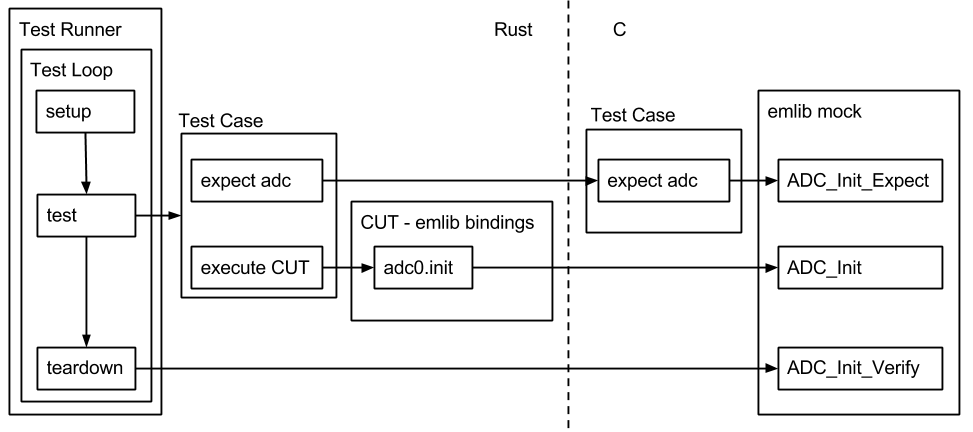
\includegraphics[scale=0.3]{figures/testframework}
  \end{center}
  \caption{Flowchart for test framework}
  \label{fig:test-framework}
\end{figure}


\subsubsection{Rust libtest}

The {\rust} programming language contains a testing framework within the standard library.
The reasons for not using it to test the bindings is that we needed to run the tests on the {\gecko}.
The rational for this is that the tests are mostly checking that the datatypes used on the {\rust} and {\C} side of the bindings are compatible.
Therefore we need to use the proper compilers and compile the test targets for the ARM platform, verifying that the platform-specific \prog{gcc} and {\rustc} have compatible types does not help in respect to this.
Consequently, {\rust}'s standard testing framework relies heavily on {\rust}'s own {\std} library, which renders the framework unusable for our embedded platform.

% Consequently, {\rust}'s standard testing framework is rendered unusable for our embedded platform because it relies heavily on the {\rust}'s own {\std} library.

% Consequently, given that the testing framework in the standard library relies heavily on the  that was discussed in \autoref{sec:back:lib}, this renders the framework unusable for our embedded platform.

\subsection{Discussion}

Writing the bindings for the different peripherals was a tedious work, that required careful review of the {\emlib} source code in order to correctly port enum- and struct-definitions from {\C} to {\rust}.
Additionally, we had to redefine many constants, like the names of memory-mapped register bit-fields like the ones presented earlier in \autoref{fig:back:memorymapped}, or values calculated from various {\C} macros defined in header files that are used throughout the library.
We had to retrieve the value of the constants by debugging the source code and explicitly look up the value of these constants if they were only implicitly defined in the header files.

Since we have constrained our library to only support the EFM32GG990 devices we chose to manually write the bindings for the library, instead of generating the bindings through some kind of automated process.
There were already a couple of tools available for generating such C-bindings automatically, that could possibly have made the process quicker.
However, we chose not to utilize such tools because of the reasons described below.

\begin{itemize}
    \item It was quick and easy to get started with code for a new peripheral.
    This argument was especially important when the project started out, because we still had no clue of how the project would evolve and what it was going to look like.

    \item It was an advantage to depend on as few third party tools as possible, since both {\rust} and all available libraries would be unstable until the 1.0 release of the language.

    \item We wanted to keep the naming convention of our bindings as similar to {\emlib} as possible, this would not have been easy to keep consistent with an automated process, partly because there are exceptions where these conventions do not fully hold.
    It is however an interesting problem that would have a higher priority if the library were ever to support more than one EFM32 device.

    \item We could focus on writing bindings for smaller parts of each module separately when we first needed them, which would split the work into smaller work-packages.
\end{itemize}



\corechapter{Build System}{build}{%
  In this chapter we step out of the core software components of the {\rg} platform to present an external but highly important part of the {\rg} platform.
  The {\cargo} package manager is an integral part of the {\rust} ecosystem and facilitates sharing code libraries with ease.
  Throughout this chapter we look at how we evolved the build system over time and ultimately migrated the process over to {\cargo}.
}
\section{Build System}
\label{sec:build_system}

Building the library and the EFM32 executables turned out to be one of the major parts of the work done in this project.
This section describes how building the project have changed over time.
This includes managing dependencies, compiling the RCL and REL and the Silicon Labs EFM32 \texttt{emlib}.
We have also utilized a continuous integration system that has helped us to keep the project up to date with the nightly builds of Rust and making sure that the builds have been consistent across the systems it has been built on.

\subsection{Early days}
\label{ssub:using_make}

\todo{Maybe mention more about armboot in background instead of here.}
When the project first started out it was based upon the \texttt{armboot} \cite{github:armboot} git repository available on GitHub.
\texttt{armboot} is a small template project for using Rust bare metal on a STM32 ARM \glspl{mcu}.
These are, similarly with the EFM32 series, also based on the Cortex-M series of ARM processor cores.

\todo{Håvard: Skriv denne seksjonen}
The project got up and running pretty fast based on how \texttt{armboot} was built.
We looked at armboot's Makefile to figure out what flags to pass to \texttt{rustc} in order to make it cross-compile for an ARM target architecture.

\subsection{Transitioning to Cargo}
\label{ssub:transitioning_to_cargo}

It was always a goal to use Cargo for building, distributing, and managing the packages and dependencies that would become part of this project.
An obvious reason for this was to lower the bar for other potential users of the library, and to make our project as standalone as possible, so that it is easier to include and extend it as a part of other potential projects.
By letting \texttt{Cargo} handle as much as possible in its build routine, it will automate a lot of the work that every programmer using the library otherwise would have to do manually

When the project first started out it was built by compiling Rust's core library and Silabs' emlib C sources separately, and then linking them with the \gls{ffi} bindings for emlib by hand.
While this approach worked, it was far from optimal for a number of reasons:

\begin{itemize}
    \item Rust was in active development and many of it's unstable \glspl{api} were going through rapid changes. Ensuring that versions of rustc and the Rust source code stayed up to date across different systems was not easy.
    \item Compiling and ensuring that all dependencies were consistent across builds and systems for the bindings were a tedious task. A lot of the troubles concerning this came back to the point above.
    \item Linking dependencies with the library required each system to have set up several different \$PATHS to point to the right directories, what worked for one developer on one system might not have worked for different developer on another system.
    \item The Cargo package manager was developed for exactly these purposes among others.
\end{itemize}

As already described, Cargo is a tool that provides many operations to build Rust projects that has a certain project structure.
It is designed to integrate with other existing tools, like GNU Make, which has been important in  building this project.
When the transition to Cargo started, we focused on structuring the main library and its modules into the directory structure described in \autoref{ssub:project_structure}.
By invoking the \texttt{cargo build --verbose} command, it was possible to see the output from what Cargo attempted to build when it failed, and then structure the project accordingly.

A big priority was to to shrink the size of the makefiles that was in the project by making them a part of the standard build process for \texttt{emlib} instead, doing this would help us get a long way of ensuring that the builds done by Cargo could be consistent across systems.
By defining a Rust build script and utilizing a Rust build-dependency called \texttt{gcc} \cite{web:cargo_gcc}, we were able to compile the C sources from Silabs' emlib and link them with our bindings directly as part of the build process.
Note that the \texttt{gcc} build-dependency is used as a shell to merely \emph{invoke} the underlying C-compiler, in our case it is used to cross-compile with the \texttt{arm-none-eabi-gcc} compiler.
By removing the dependency of manually compiling the C sources, it was easier to start to automatically fetch the other dependencies like the \texttt{core} and \texttt{collections} libraries.

Because the project is for a different processor architecture than the system that it is built on, we had to conditionally cross-compile all the standard Rust libraries that we wanted to utilize for the ARM Cortex-M3.
We could not utilize the pre-compiled libraries that are already included with \texttt{rustc}, since these only works for the current system architecture.
\todo{Mention this in discussion. Is there a better way of solving this? Currently it fetches a release tarball of the language. It fetches more than it needs to for each library, but it's quicker/easier than using e.g. git to do it. It does however take a little while to compile all the dependencies on smaller machines.}
We solved this problem by implementing a new Cargo build-dependency, called \texttt{rust-src} \cite{github:rust_src}, whose purpose is to download the entire Rust source code that is compliant with the instance of \texttt{rustc} that is \emph{currently} compiling the library.
By making it a task for each build to fetch its own source code, we were guaranteed that the dependencies we used for the project would always compile, independent of the current instance of \texttt{rustc} that was installed on the system.
\autoref{tab:compiled_libraries} summarizes the different crates that we have fetched from Rust's standard library in order to use them with our project.
\todo{May not need this table here. Need to synchronize with the section that presents REL and such..}

\todo{We need to write about the \texttt{rlibc} crate, and the need to define our own \texttt{memmove} and \texttt{memalign} functions in order to use alloc (Box, Vector, ...)}

\begin{table}[ht]
\begin{center}
\begin{tabular}{r|p{8cm}}
\textbf{Rust library} & \textbf{Purpose} \\
\hline
core        & Rust's core library that declares basic types. \\
libc        & Types to use with Rust's \gls{ffi}. \\
alloc       & Allows for heap-allocated variables. \\
collections & Provides common collections like dynamically allocated Strings and Vectors. \\
unicode     & Required by collections for e.g. Strings. \\
rand        & Generate random values. \\
\hline
\end{tabular}
\caption{Rust libraries conditionally compiled for the Cortex-M3 architecture.}
\label{tab:compiled_libraries}
\end{center}
\end{table}

By design Cargo only supported passing two flags further on to \texttt{rustc}, those were \texttt{-L} and \texttt{-l}, their purpose is to tell \texttt{rustc} to link with an external library by looking in a directory (specified with the \texttt{-L} flag), for a library with the specified name (specified with the \texttt{-l} flag).
The last step in the build process involved linking \texttt{emlib} and the other libraries with an actual executable for the Cortex-M3.
This was not possible to do with Cargo since it required us to pass a couple of extra linker-flags further on to \texttt{rustc}.
\todo{Håvard: Jeg har ingen anelse over hvor riktig dette er. Noe av dette blir vel beskrevet et annet sted, vi får finne en måte å referere til riktig seksjon her, uten å gå altfor mye i detalj...}
The flags were needed by \texttt{rustc} in order to tell it to link with an external library for a different architecture and to include a separate linker-script that took care of booting up the executable on this architecture.

Another issue that was introduced by automatic compilation with Cargo, was how it structured the packages it compiled.
When Cargo builds a project and its dependencies it structures all the generated metadata and the compiled libraries within a \texttt{target} directory, and an extra filename gets appended to all of these libraries.
This extra filename is part of a hash that is generated based on the code in the library, and ensures that each and every build is consistent and it resolves any problems that might arise if several dependencies within a project depends on different versions of the same library.
This works when Cargo handles the entire build process, but it our case, where we had to manually compile the final executable, it turned out to be a problem because the name of the library would change every time some of its content changed.
We worked around this problem by modifying the build script to store the hash generated by Cargo for \texttt{emlib} to a text file, every time the library was built, and then included it in the makefile for the project.

\subsection{Conditional linking with Cargo}

The build process described in the previous section made it simpler to use third party libraries, but it did not solve all of our issues, the main problem that persisted was to have a good way of making \texttt{emlib} itself, portable.
With the setup that we had, it was easy to create new executables \emph{within} the project, but it was hard to create new executables that \emph{depended} on \texttt{emlib}.
Basically, because we had to work around Cargo in the final part of the build process, it also meant that \emph{every} project that wanted to depend on \texttt{emlib} also had implement the same workarounds.
Thus, we needed to solve the problem of knowing where Cargo would store the project metadata, and we needed a way to get Cargo to compile the final executables with the extra linker-arguments needed by \texttt{rustc} in order to compile the binary for the Cortex-M3.

Cargo does not have much documentation over how its internal works, or how to interfere with the build process, but the documentation does mention that Cargo can be extended with additional \emph{plugins}.
If Cargo is to be invoked with a command that it does not have by default, it will query the system for this command.
This means that if Cargo is invoked with e.g. the command \texttt{cargo foo <args>...}, it will query the system for an executable with the name \texttt{cargo-foo} and it will invoke this command with the trailing arguments if it exists.
By looking at Cargo's source code, we could see that every triggered build included a structure called \texttt{CompileOptions}.
The arguments passed to Cargo's different build commands are then used to compose this structure and trigger an internal compilation process, this process handles the compilation of all dependencies and generates all the different targets for the current package to be compiled.
\todo{Would it be nice with some kind of figure that describes the build process?}

\begin{table}[ht]
\begin{center}
\begin{tabular}{r|p{8cm}}
\textbf{Flags} & \textbf{Purpose} \\
\hline
\texttt{[$<$args$>$]} &
The trailing argument to the command was the linker-arguments that was to be passed further on to the invocation of \texttt{rustc}.
If any \texttt{args} are present, Cargo will append \texttt{-C link-args="$<$args$>$"} when any executables from the package package is being built. \\

\texttt{--examples NAME} &
The library had many executables located in the projects \texttt{examples} directory.
This flag made it easier to compile one of these examples by specifying its name. \\

\texttt{--build-examples} &
This flag filtered out every executable marked as an example and compiled all of them. \\

\texttt{--print-link-args} &
This flag was included for debugging purposes. \\

\hline
\end{tabular}
\caption{}
\label{tab:cargo_linkargs}
\end{center}
\end{table}


In order to solve the problems we had with building the project, we created a new subcommand called \texttt{cargo-linkargs} \cite{github:cargo_linkargs} that depends on Cargo itself.
This subcommand was created specifically with \texttt{emlib} in mind, and supports all the flags that the \texttt{cargo-build} command supports, including the flags shown in \autoref{tab:cargo_linkargs}.
We got rid of the two problems we had with building \texttt{emlib} once \texttt{cargo-linkargs} was working.
The problem with resolving the location of generated metadata were solved implicitly just by utilizing Cargo, and the extra linker-arguments could easily be passed on to the invocation of \texttt{cargo-linkargs} via the project's makefile.

\subsection{Continuous Integration}
\label{ssub:continuous_integration}

When we first started this project, Rust had reached a 1.0-alpha version.
This meant that the programming language had reached a relatively stable state, but there was still big parts of the language and its standard libraries that was marked as unstable and up for review before the planned 1.0 release.
The standard libraries, and third party Rust libraries that has evolved in the Rust community, have made little guarantee about their stability, and the \glspl{api} have been subject to change without much notice.

Continuous Integration refers to the practice of testing the whole system \emph{continuously}, for every smaller change introduced to the code base, usually with some kind of automated test framework.
Continuous Integration is advantageous to normal regression testing because it can reduce the amount of code rework that is needed in later phases of development, as well as speed up overall development time  \cite{Orso2014}.
Many Rust projects have utilized a continuous integration system called Travis CI \cite{web:travis_ci} for ensuring that the code in the project have been compatible with the nightly builds of Rust.
By registering our projects with Travis CI, and a community-developed service called Rust CI \cite{web:rust_ci}, we had automatic, daily builds of our projects on a third-party server.
Builds were triggered every time we released a change to the code on GitHub, and every time a new nightly release of Rust was published, and if a build failed we would get notified of the error.
By making continuous integration part of the normal build routine and review-process for new project code, we had an extra step of verification that the project would build on other systems then the one it was developed on.

It is important to note that continuous integration only helped us to verify that the project could be \emph{built}, it could not help us to verify that the compiled code would actually \emph{work} for its target architecture.
In order to verify that the code would work for on the Cortex-M3 we had to actually run in on one of the microcontrollers that we had a available for this project.
An experimental process of testing and mocking the \texttt{emlib} \gls{api} bindings is described in greater detail in \autoref{ssub:testing}.

\subsection{Contributing to Cargo}
\label{ssub:contributing_to_cargo}

As already mentioned, the ability to pass arbitrary flags down to the invocation of \texttt{rustc} was by design not supported by Cargo, but many people in the Rust community have wanted the ability to do so.
The reasoning for not allowing arbitrary flags to be passed down is pretty obvious.
A compilation can go awry very quickly if it is up to the package \emph{author} what flags should be passed to \texttt{rustc} instead of the package \emph{builder}.
This would give the author the ability to set the restriction for a library, not the user.
Different systems do not necessarily support all flags and possibilities, so if a package dependency says that it is to be built in a specific way it might not work for the system that is building it.

There have been an issue on Cargo's project page about implementing a new subcommand (called \texttt{cargo-rustc}) for the package manager.
This subcommand would have allowed for passing arbitrary flags further on to \texttt{rustc}, but with the restriction of only compiling a \emph{single} target at a time.
This means that only \emph{either} the library, a binary, an example or a test (or a package dependency), may be compiled with the extra flags, and \emph{not} the entire package.
These rules are restrictive enough to get libraries to not depend on a set of extra flags, but loose enough so that specialized projects, like our \texttt{emlib}, can depend on it for completing the build.
Indeed, the functionality proposed with this subcommand would be enough to cover all the cases that we solved with our implementation of \texttt{cargo-linkargs}.

After gaining insight into Cargo's internals during the development of \texttt{cargo-linkargs}, it was interesting to see if we could get this same functionality into Cargo itself by implementing \texttt{cargo-rustc}.
Not only would it benefit our project, it would also give many other Rust projects the ability to use Cargo for the entire compilation process.
Since both Rust and Cargo are open source projects, it was easy to get in contact with the project maintainers about the issue, and eventually submit a pull-request with the new subcommand.
After it was reviewed by one of the project maintainers, the pull-request was accepted and merged into Cargo's code base.


\corechapter{Application Layer}{app}{%
  In the Application Layer module of the {\rg} platform we find the application level libraries and actual executable programs.
  As part of this chapter we have included some experimental libraries developed to explore the language facilities of the {\rust} programming language in an embedded system.
  We also look at two projects developed for providing a qualitative study of the platform.

  All of the programs and libraries presented in this section builds upon the foundation provided by the lower levels of the {\rg} platform.
  None of these components are mandatory when using the platform, and when writing an application using this platform that code itself is considered part of this layer.
  The components in the following section represent example applications and possible future extentions to the base {\rg} platform as given by the previous sections.
}
\subsubsection{Closures as interrupt handlers}
\label{sec:irq-closures}

This section describes an experimental approach to handling interrupts with closures.
The motivation for using this pattern to make the code more Rust ideomatic and to make use of the ownership rules applied to closures.
The Rust programming language frowns upon using global variables, especial when the variables are mutable.
Using such variables forces the programmer to use unsafe blocks thus transfering the responsibility of the safety analysis from the compiler to the programmer.
Therefore avoiding mutable global state is a goal of any Rust program.

\paragraph{Motivation}
\label{par:irq:motivation}

Lets consider a simple example for motiviating the use of closures to handle interrupts.
The example application samples an analogue signal and saves the result to a memory buffer.

\begin{listing}[H]
  \begin{minted}{rust}
// Declaring a Circular Buffer Type globally
const N: usize = 1024;
static mut IDX = 0;
static mut BUFFER: [u32; N] = [u32; N];

fn main() {
  let adc = adc0();
  // Using BUFFER requires unsafe
  // e.g.: unsafe { &BUFFER[..] }
  loop {}
}

pub extern fn ADC0_IRQHandler() {
  let adc = adc0();
  let sample = adc.get_single_data();
  // Writing to the buffer is considered unsafe
  unsafe { BUFFER[IDX % N] = sample; }
}
  \end{minted}
  \caption{Analogue sample with global buffer}
  \label{lst:irq:global}
\end{listing}

\autoref{lst:irq:global} shows an example of the proposed example with a conventional interrupt handler.
The interrupt handler is in the global scope, so it can only access global variables and therefore the buffer must be declared as \textbf{static mut}.
This require all read and writes to the buffer to be contained within unsafe blocks.
A huge restriction on variables defined in the global scope in Rust is they can only be of types which has constant-expression constructors.
This is a fact which we praised in \autoref{sec:impl:booting} as it provides a very simple startup procedure but it limits the datatypes which can be shared between interrupt handlers and the rest of the code.

\begin{listing}[H]
  \begin{minted}{rust}
fn main() {

  let mut adc = adc0();

  let buffer = CircularBuffer::new();
  let mut ch = buffer.in();

  // Register a closure on the ADC
  // The closure will be called each time
  // a new sample is ready with the sample
  // as an argument.
  // The move keyword is used to move ownership
  // of the ch cariable
  adc.on_single(move |sample| ch.send(sample));

  // Reading from buffer is safe
  // e.g.: &buffer[..];
  loop {}
}
  \end{minted}
  \caption{Analogue sample with local buffer}
  \label{lst:irq:local}
\end{listing}

In \autoref{lst:irq:local} we present an example implementation using a closure as an interrupt handler.
The global state is now replaced with a buffer which is owned by the main function stack frame.
In this discussion we consider the \textbf{main} stack frame, the stack fram for the main function, as a special frame.
This comes by the fact that the main function contains an infinite loop causing it to never terminate and the frame will not get deallocated.
On an embedded system this is true as long as a fatal error does not occure.
So we can relie on variables owned by the main stack frame to live for the duration of the application.
This ensures that the \textbf{buffer} for pratical purposes has the same lifetime as the \textbf{BUFFER} from \autoref{lst:irq:global}, but the fact that the variable is not a \textbf{static mut} lets the programmer avoid \textbf{unsafe} blocks and let the compiler ensure safety.
One implementation detail here is the imangined \textbf{CircularBuffer} type.
The type is based on the same principal as the Rust standard library \textbf{channel} type, which provides a facility for interprocess communication.
The channel has one \textit{read end} and one \textit{write end} enabling the producing process to send a stream of messages to the consuming process.
This is required for the \gls{adc} callback to be able to write to the buffer while the main function retains ownership of the buffer.
In the example the \texttt{in} function creates the \textit{write end} of the circlar buffer.

The core of this example is the line \texttt{adc.on\_single(move |sample| ch.send(sample));}.
This creates a closure which takes ownership over the \textit{write end} for the circular buffer.
The closure is passed as a argument to the \texttt{on\_single} method on the \gls{adc} ensuring that the closure is called each time a new sample is ready with the sample as an argument.

\paragraph{Implementation}
We now look at how we can provide this behaviour in Rust and present the problems that arised along the way.

The process of handling an interrupt is described in \autoref{sec:impl:handling-interrupts}.
In order to implement the pattern above we need to get the globally defined interrupt handler \texttt{ADC0\_IRQHandler} to call a closure created in the main function.
So lets first consider what a closure is.
A closure is the \textbf{environment} it closes over, in \autoref{lst:irq:local} the \texttt{ch} variable, and a \textbf{function pointer}, that simple.
See \autoref{sec:back:rust:closures} for additional details of closures.

An initial naive idea of registering the function pointer from the clousre in the interrupt vector will not work as the function nees to be called with the environment in the closure.
Therfore we need to store the whole closure in a datastructure and ensure that it is called by the interrupt handler.
First we try to store the closure in a global datastructure which the handler can access as implemented in \autoref{lst:global-closure}.

\begin{listing}[H]
  \begin{minted}{rust}
static mut CLOSURE: Option<Fn()> = None;
  \end{minted}
  \caption{Storing the closure globally}
  \label{lst:global-closure}
\end{listing}

In \autoref{lst:global-closure} we introduce the \texttt{Fn} trait.
This is a trait which a represent closure in Rust.
Wrapping the closure in an \texttt{Option} is done to enable the handler to be undefined.
Compiling this will yield an error due to the fact that the compiler cannot statically determine the size of the closure and therefore does not know how much memory to allocate.
This problem occures quite common in programming and the default solution is to put the value behind a pointer as shown in \autoref{lst:global-pointer-to-closure}

\begin{listing}[H]
  \begin{minted}{rust}
static mut CLOSURE: Option<Box<Fn()>> = None;
  \end{minted}
  \caption{Storing a pointer to the closure globally}
  \label{lst:global-pointer-to-closure}
\end{listing}

This introduces a Box which yields an indirection, storing the closure on the heap.
Unfortunatly this does not make the program compile.
It is due to the fact alluded to earlier saying that global variables cannot have a type which does not have a constant-expression initializer.
The Box type is one of these types which are disallowed as global variables.

To get around this issue we need to use raw pointers.
We substitue the \texttt{Box} pointer with a raw pointer to the closure as shown in \autoref{lst:raw-global-pointer-to-closure}.

\begin{listing}[H]
  \begin{minted}{rust}
static mut CLOSURE: Option<*const Fn()> = None;
  \end{minted}
  \caption{Storing a pointer to the closure globally}
  \label{lst:raw-global-pointer-to-closure}
\end{listing}

Now we've managed to store a closure in a statically allocated location.
\autoref{lst:pub-sub} shows a safe abstraction to register and dispatch events with this handle.

\begin{listing}[H]
  \begin{minted}{rust}
// Registers an interrupt handler
fn register(f: Box<Fn()>) {

  unsafe {

    // Deallocate old handler if existing
    match CLOSURE {
      Some(old) => {
        // Remove the global reference
        CLOSURE = None;

        // Return the ownership of the pointer
        // to a managed box, this will ensure
        // that the contents is deallocated when
        // the box variable goes out of scope
        let box= boxed::from_raw(old);
      },
      None => ()
    }

    // Consume the Box pointer and
    // return a raw pointer to the closure
    let raw = boxed::into_raw(f);

    // Save the closure pointer in the global reference
    CLOSURE = Some(raw);
  }

}

// Dispatch a event by calling the closure if it is registered
fn dispatch() {

  // The Closure is stored in a global variable mutable
  // So the access to this variable is unsafe
  match unsafe { CLOSURE } {

      // Unwrap the closure value
      Some(func) => unsafe {

        // The closure is stored behind a pointer which must
        // be dereferenced, it is called with is environment
        // by invoking the function: call
        (*func).call(())
      },
      None => ()
    }
  }
}
  \end{minted}
  \caption{Safe abstraction over global reference}
  \label{lst:reg-disp}
\end{listing}

As discussed in the beginning of this section the Gecko provides a vector of interrupts.
The design for the closure described this far is only capable of storing a single closure.
We now alter the design to handle an arbritrary number of handlers.

First we define two datatypes which will aid our implementation.
The Event enumeration given in \autoref{lst:enum:Event} which mirrors the interrupt handlers defined in the interrupt vector and an event hub structure shown in \autoref{lst:struct:Hub}

\begin{listing}[H]
  \begin{minted}{rust}
enum Event {
    ADC0,
    TIMER0
    // mirrors interrupt vector
}
  \end{minted}
  \caption{Enumeration for Irq Handler Tag}
  \label{lst:enum:Event}
\end{listing}

\begin{listing}[H]
  \begin{minted}{rust}
// Datastructure with a Binary Map from Event to handler
struct Hub {
  handlers: BTreeMap<Event, Box<Fn()>>
}

// Signatures for implementation of the Event Hub
impl Hub {

  // Create an empty hub
  fn new() -> Hub { /* .. */ }

  // Register a handler for an Event
  fn register(&mut self, event: Event, f: Box<Fn()>) { /*...*/ }

  // Trigger an event
  fn dispatch(&self, event: Event) { /*...*/ }
}

// We do not want users to interact with the hub directly so we provide
// a public interface for registering and dispatching events
pub fn register(event: Event, f: Box<Fn()>) { /*...*/ }
pub fn dispatch(event: Event) { /*...*/ }
  \end{minted}
  \caption{Event Hub structure}
  \label{lst:struct:Hub}
\end{listing}

And finally the interface used in \autoref{lst:irq:local} is created using the utilities \texttt{register} and \texttt{dispatch}.
\begin{listing}[H]
  \begin{minted}{rust}
impl Adc {

  // This constructor is defined in emlib
  pub fn adc0() -> &'static Adc { /*...*/ }

  pub fn on_single(&'static self, callback: Box<Fn(u32)>) {

    // Make sure the callback for
    // a single conversion is enabled
    self.int_enable(IEN_SINGLE);

    // Call the utility to register a irq handler
    // The move keyword is used to move
    // ownership of the callback function into the closure
    register(Event::ADC0, Box::new(move || {

      // Clear interrupt signal to mark it as handled
      self.int_clear(IF_SINGLE);

      // Call the interrupt handler with the ADC sample
      callback(self.data_single_get())
    }));
  }

  // Clears interrupt signals
  pub fn int_clear(&self, flag: u32) { /*...*/ }

  // Retreives next sample from the ADC
  pub fn data_single_get(&self) -> u32 { /*...*/ }
}

// The ADC0 Interrupt handler
// This is defined as a part of the library
#[allow(non_snake_case)]
fn ADC0_IRQHandler() {
    dispatch(Event::ADC0);
}
  \end{minted}
  \caption{Storing a pointer to the closure globally}
  \label{lst:raw-global-pointer-to-closure}
\end{listing}

Now looking back at out target implementation in \autoref{lst:irq:local} we augment the example to be functional with the library presented in this section.

\paragraph{Working example with closure as interrupt handler}

\autoref{lst:irq:closure} shows a runnable version of the example application from \label{par:irq:motivation}.

\begin{listing}[H]
  \begin{minted}{rust}
fn main() {

  // Create Event Hub and save it to the global variable
  let mut hub = Hub::new();
  unsafe { HUB = Some(&mut hub); }

  let mut adc = adc0();
  let buffer = CircularBuffer::new();
  let mut ch = buffer.in();

  adc.on_single(Box::new(move |sample| ch.send(sample) });

  // Using buffer is safe
  // e.g.: &buffer[..];
  loop {}
}
  \end{minted}
  \caption{Analogue sample with local buffer}
  \label{lst:irq:closure}
\end{listing}

The changes in \autoref{lst:irq:closure} compared to the \autoref{lst:irq:local} is the callsite of registering the cloures where it is passed inside of a owning Box pointer. \todo{We should be able to pass it by value as std::thread::spawn does}
The other more significant change is the creation and registration of the \texttt{hub} variable, it is also stored in the global variable defined in \autoref{lst:struct:Hub}.
This code pattern is highly risky and must be used with great care.
The method allocates an object on the stack and saves a mutable reference to it in an global variable.
If this technique is utilized on an arbitrary stack frame and the reference is read from, the program will most probably crash.
This is because the stack frame in question will probably be deallocated and either unused or used for another stack frame.
As mentioned in the start of this section we consider the stack frame of the main function as a special frame which will not be subject for deallocating, unless the application is about to terminate.
This ensures that the \texttt{hub} variable has \texttt{static} lifetime and can be used store the boxed closures while still being reachable from the global reference \texttt{HUB}.
The inspiration for this \textit{hack} was drawn from the pattern being used in the Servo project for setting up an Event Loop.

Elimintaing the main stack frame dependence was considerable easy to do by using the same conversion used in the register call above.
\autoref{list:irq:init} shows a initializing function which creates a \texttt{Hub} object and registrers it in the \texttt{HUB} reference.

\begin{listing}[H]
  \begin{minted}{rust}
pub fn init() {

  if unsafe { HUB.is_none() } {
    let hub = Box::new(Hub::new());
    let raw = unsafe { boxed::into_raw(hub); }
    unsafe { HUB = Some(raw); }
  } else {
    // already registered so ignore the call
  }
}
  \end{minted}
  \caption{Saving a global reference to a heap allocated object}
  \label{lst:irq:closure}
\end{listing}

% !TEX root = ../main.tex

\section{Porting GPIO Interrupt Driver}
\label{sec:porting-gpioint}

This section considers a case study of an issue in the {\emdrv} library, and it was discovered while we ported the \gls{gpio} interrupt driver from {\C} to {\rust}.
This driver was ported to {\rust} because we wanted to issue \gls{gpio} interrupts with {\rust} function pointers, without needing to declare them with the {\C} \gls{abi} (which was required by {\emdrv}).
The issue was discovered when annotating the \texttt{unsafe} blocks for referencing mutable global state, and gives an example of the awareness the inclusion of the {\unsafe} keyword provides.

\subsection{Presenting the Problem}

The \texttt{gpioint} driver lets the user register a callback function to be called when an interrupt occurs at a given \gls{gpio} pin.
It is implemented with a global mutable list of 16 function pointers, a register function to assign functions to indices of the list corresponding to the \gls{gpio} pins, and a dispatch mechanisms which calls the correct functions when an interrupt occurs.
The issue arises in the dispatch function in \autoref{lst:irq-dispatch:c}.

\begin{listing}
  \begin{ccode}
static void GPIOINT_IRQDispatcher(uint32_t iflags) {
  while(iflags) {
    // Utility for iterating through all active interrupt signals
    uint32_t irqIdx = GPIOINT_MASK2IDX(iflags);
    // Mark interrupt as handled
    iflags &= ~(1 << irqIdx);
    // Check if the interrupt has a callback
    if (gpioCallbacks[irqIdx]) {
      // Call the callback
      gpioCallbacks[irqIdx](irqIdx);
    }
  }
}
  \end{ccode}
  \caption{GPIO Dispatcher from {\emlib}}
  \label{lst:irq-dispatch:c}
\end{listing}

\begin{listing}
  \begin{rustcode}
static mut GPIO_CALLBACKS: [Option<fn(u8)>; 16] = [None; 16];

fn dispatcher(iflags: u32) {
  while(iflags) {
    // Utility for iterating through all active interrupt signals
    let irq_idx = mask_to_index(iflags);
    // Mark interrupt as handled
    iflags &= !(1 << irq_idx);
    // Check if the interrupt has a callback
    if (unsafe { GPIO_CALLBACKS[irq_idx] }.is_some()) {

      // Window of opportunity

      // Unwrap the callback and call the function
      unsafe { GPIO_CALLBACKS[irq_idx] }.unwrap()(irq_idx);
    }
  }
}
  \end{rustcode}
  \caption{GPIO Dispatcher naively ported to {\rust}}
  \label{lst:irq-dispatch:rust}
\end{listing}

A first take at porting the dispatcher function to {\rust} yields the code in \autoref{lst:irq-dispatch:rust}.
It is quite easy to see that the global mutable state is read twice exposed by the compiler requirement to include the {\unsafe} keyword.
This means that there is a possibility of the second reference to return a different value than the first.
For instance the function \func{GPIOINT\_CallbackUnRegister(uin32\_t pin)} will set the function pointer in the array to \mem{0x0} for the specified pin.
If this function is called inside a interrupt handler and this interrupt is triggered while the GPIO driver is dispatching an interrupt, the function pointer can be set to \mem{0x0} between the check and the call.
Calling a function pointer that points to \mem{0x0} will cause a \func{HardFault}.

\subsection{Analysis of Assembly}
To dive a bit further into the issue and to prove that it is only present at optimization level O0 we consider the assembly code, generated by compiling the {\C} source, for the dispatcher.

The subsection of the \func{GPIOINT\_IRQDispatcher} in assembly generated by \prog{arm-none-eabi-gcc -O0 -S} is reproduced in \autoref{lst:gpio:asm:O0}.

\begin{listing}[H]
  \begin{ca65code}
GPIOINT_IRQDispatcher:
  ;; ...                    ;;
  ldr r3, .L34              ;; r3 = gpioCallbacks
  ldr r2, [fp, #-8]         ;; r2 = irqIdx
  ldr r3, [r3, r2, asl #2]  ;; r3 = gpioCallbacks[irqIdx]
; start interrupt window    ;;
  cmp r3, #0                ;; if (r3 == 0) {
  beq .L30                  ;;
  ldr r3, .L34              ;;   r3 = gpioCallbacks
  ldr r2, [fp, #-8]         ;;   r2 = irqIdx
; end interrupt window      ;;
  ldr r3, [r3, r2, asl #2]  ;;   r3 = gpioCallbacks[irqIdx]
  ;; ...                    ;;
  bx  r3                    ;;   (*r3)();  call the function
  ;; ...                    ;; }
  \end{ca65code}
  \caption{GPIOINT Dispatcher in assembly with O0}
  \label{lst:gpio:asm:O0}
\end{listing}

Here we see a window of 4 instructions where the proposed harmfull interrupt can occur.
It is the \func{ldr} instruction just before the window opening and the one just after that causes the issue.
These two loads must load the same address for the logic to be valid, although the second one is just required to not load \mem{0x0} in order not to cause a \func{HardFault}.

Looking at the same assembler generated by compiling the code with \prog{arm-none-eabi-gcc -O1 -S} in \autoref{lst:gpio:asm:O1} we see that the issue has been eliminated.

\begin{listing}[H]
  \begin{ca65code}
GPIOINT_IRQDispatcher:
  ;; ...                    ;;
  ldr r5, .L5               ;; r5 = gpioCallbacks
  ;; ...                    ;;
  and r3, r0, #255          ;; r3 = irqIdx
  ;; ...                    ;;
  ldr r3, [r5, r3, asl #2]  ;; r3 = gpioCallbacks[irqIdx]
  cmp r3, #0                ;; if (r3 == 0) {
  ;; ...                    ;;
  bxne    r3                ;;   (*r3)()
  ;; ...                    ;; }
  \end{ca65code}
  \caption{GPIOINT Dispatcher in assembly with O1}
  \label{lst:gpio:asm:O1}
\end{listing}

At O1 the compiler has performed \gls{cse} to remove the duplicate load present in \autoref{lst:gpio:asm:O0}.
This can be elimintated with the assumption that the \code{gpioCallbacks} will not be changed by external code.
But as the {\rust} version in \autoref{lst:irq-dispatch:rust} suggests this code can lead to a \concept{data race} because it is referencing a global mutable variable.

\subsection{Proposed solution}

The solution to this problem is quite straightforward by performening the \gls{cse} manually.
\autoref{lst:irq-dispatch:c-fixed} contains the implementation proposed to Silicon Labs to resolve this issue.

\begin{listing}[H]
  \begin{rustcode}
static void GPIOINT_IRQDispatcher(uint32_t iflags) {
  while(iflags) {
    uint32_t irqIdx = GPIOINT_MASK2IDX(iflags);
    iflags &= ~(1 << irqIdx);
    GPIOINT_IrqCallbackPtr_t callback = gpioCallbacks[irqIdx];
    if (callback) {
      callback(irqIdx);
    }
  }
}
  \end{rustcode}
  \caption{GPIOINT Dispatcher without Data Race}
  \label{lst:irq-dispatch:c-fixed}
\end{listing}

We again consult the assembly code in \autoref{lst:irq-dispatch:asm-fixed} generated to verify that this resolved the issue.

\begin{listing}[H]
  \begin{ca65code}
GPIOINT_IRQDispatcher:
  ;; ...                     ;;
  ldr   r3, .L34             ;; r3 = gpioCallbacks
  ldr   r2, [fp, #-8]        ;; r2 = irqIdx
  ldr   r3, [r3, r2, asl #2] ;; r3 = gpioCallbacks[irqIdx]
  ;; ...                     ;;
  cmp   r3, #0               ;; if (r3 == 0) {
  ;; ...                     ;;
  bx    r3                   ;;   (*r3)()
  ;; ...                     ;; }
  \end{ca65code}
  \caption{GPIOINT Dispatcher for proposed solution at O0}
  \label{lst:irq-dispatch:asm-fixed}
\end{listing}

\subsection{Discussion}

The issue presented in this section is a minor one and will probably never cause a \func{HardFault} in a real world application.
Nevertheless is serves as an example of how the {\unsafe} keyword in {\rust} makes the programmer think twice about code in these unsafe sections.
It also points to the gains of using {\rust} to prototype subsets of an C library to see if issues with a more strict compiler will arise from the patterns and constructs used.

% !TEX root = ../main.tex

\section{Rust Embedded Modules}
\label{sec:rust-embedded-modules}

This section describes a separate project, which we refer to as \gls{rem}.
\gls{rem} have been developed alongside the implementation of the various binding libraries, and contains a handful of higher-level modules for {\emlib}'s different peripheral bindings.
The peripheral abstractions that have been implemented as part of \gls{rem} are still in very early development

\subsection{Peripheral Abstractions}
\label{sub:peripheral_abstractions}

 % and act as playground to experiment with how {\rust} can be used to define high-level

This section describes the different peripheral abstractions that are part of \gls{rem}.
Some of these modules are more complete than others.

\subsubsection{Usart}
\label{ssub:usart}

The \gls{usart} have many different use-cases, it is a peripheral that is used for transferring of data, but it is also a very convenient tool to use for simple debugging of programs.
It can be used to send single strings of text between a PC and the \gls{mcu}, which is convenient for ``println''-debugging, and it is a good tool for defining \gls{cli} programs.

The {\gecko} has a total of three different \glspl{usart} which can be configured to run on a total of eleven different locations i.e. \gls{gpio} Ports and Pins.
If the \gls{gpio} configuration for a \gls{usart}  is not specified correctly, the peripheral will not function correctly either.
The goal of the \gls{usart} abstraction was to make it easy to initialize the peripheral, as well as providing simple methods to read and write strings, and transfer data between two end-points.

The \texttt{Usart} module has an initialization procedure that takes care of initializing its required \gls{gpio} pins based on a specified location.
This is similar to the approach made by {\zinc}, but instead failing with a compilation-error if it is incorrectly configured, as in {\zinc}, it will fail at run-time.
A minimal example that shows how to initialize an \gls{usart}, and send and receive strings, is shown in \autoref{lst:usart_abstraction}.
Note that the example is simplified slightly, we have trimmed away some \code{extern} and \code{use} statements in order to make the important parts more clear.
The point of this example is to demonstrate a program that initializes and uses an \gls{usart} with only four lines of code.

\begin{listing}[H]
  \begin{minted}{rust}
extern crate emlib;         // Include emlib bindings
extern crate modules;       // Include `REM'
use modules::Usart;         // The USART module

#[no_mangle]
pub extern fn main() {
  // Acquire a USART with default configuration...
  let mut usart: Usart = Default::default();
  // ... and initialize its GPIO.
  usart.init_async();

  loop {
    // Perform a blocking read operation...
    let name = usart.read_line();
    // ... and echo back with a nice message.
    usart.write_line(&format!("Thank you, {}!", name));
  }
}
  \end{minted}
  \caption{Example usage of \gls{rem}'s \gls{usart} module.}
  \label{lst:usart_abstraction}
\end{listing}

\subsubsection{GPIO} % (fold)
\label{ssub:gpio}

The \gls{gpio} peripheral are used extensively as a dependency for many other peripherals throughout {\emlib}.
The microcontroller's \gls{cpu} pins are configurable as \gls{gpio}, all these pins are ordered into 10 ports (Port A - Port H) with up to 16 pins each (Pin 0 - Pin 15).
The pins can be configured individually to be used as input, output, or both, to the \gls{mcu}.

The \gls{gpio} module in \gls{rem} consists of a \code{GpioPin} structure, and two traits for \code{Button}'s and \code{Led}'s, respectively.
The \code{GpioPin} is an abstraction on top of {\emlib}'s \gls{gpio} definition, and the two traits implements a few convenient methods that abstracts away the underlying \code{GpioPin}.
An example that shows how to initialize and use a button and a LED on the {\STK} is shown in \autoref{lst:gpio_abstraction}.
Notice from the code that we only ever interfere directly with the two traits, and that we do not really care about the underlying \code{GpioPin}, apart from when we define the button and the LED.

It is important to note the \emph{current} limitations of this module.
The two implemented traits provides an intuitive abstraction layer for their purposes, but \gls{gpio} in general is so much more than just buttons and LEDs.
The module was first developed for buttons and LEDs because they are easy to interface with, but it will require some alteration in order to be more `general purpose'.

\begin{listing}[H]
  \begin{minted}{rust}
extern crate emlib;         // Include emlib bindings
extern crate modules;       // Include `REM'
use emlib::gpio::Port;
use modules::{GpioPin, Button, Led};
// Define a button and a LED. The 'static lifetime tells
// us that BTN and LED is alive for the whole program
const BTN: &'static Button = &GpioPin { port: Port::B, pin: 9 };
const LED: &'static Led    = &GpioPin { port: Port::E, pin: 2 };

#[no_mangle]
pub extern fn main() {
    // Initialize the underlying GPIO pins
    BTN.init();
    LED.init();
    // Register a callback function for the button
    BTN.on_click(blink_led);
    loop {}
}
// This function gets called when the button is pressed
fn blink_led(_pin: u8) {
    LED.toggle();
}
  \end{minted}
  \caption{Example usage of \gls{rem}'s \gls{gpio} module.}
  \label{lst:gpio_abstraction}
\end{listing}

\subsubsection{DMA}

The \gls{dma} peripheral on the {\gecko} is used for transferring data from one location to another without intervention from the \gls{cpu}.
The interface to the \gls{dma} provided by {\emlib} is a low level API which deals with hardware descriptors and raw pointers for controlling the \gls{dma}.
Here we look at a higher level abstraction over the \gls{dma} module which considers devices and buffers and the specification of the flow between these devices.

The core of the approach defines two types of endpoints which can be interacted upon with \gls{dma}, \emph{readable} and \emph{writable}.
In this classification, an \gls{adc} is readable as it produces samples and the \gls{dac} is writable as it can consume samples.
An \gls{usart} fits both descriptions, this is because data can both be written to and read from the peripheral.
Both descriptions does also apply to memory allocated buffers.

These abstractions are modeled by providing the two \keyword{traits} \code{Readable} and \code{Writable} as shown in \autoref{lst:dma:traits}.

\begin{listing}[H]
  \begin{minted}{rust}
trait Readable {
  fn as_ptr(&self) -> *mut c_void;     // Base pointer to device
  fn inc_size(&self) -> dma::DataInc;  // Increment in bytes (0, 1, 2 or 4)
  fn size(&self) -> dma::DataSize;     // Element size in bytes (1, 2 or 4)
  fn n(&self) -> Option<u32>;          // Number of elements to transfer
}
trait Writable {
  fn as_ptr(&self) -> *mut c_void;
  fn inc_size(&self) -> dma::DataInc;
  fn size(&self) -> dma::DataSize;
  fn n(&self) -> Option<u32>;
}
  \end{minted}
  \caption{Traits used for \gls{dma} transfers}
  \label{lst:dma:traits}
\end{listing}

Both \keyword{traits} defined in \autoref{lst:dma:traits} requires the same set of methods.
These methods are required by the underlying \gls{dma} implementation and are described in the {\emlib} documentation for \gls{dma}.
As mentioned, both \keyword{traits} can be applicable for some peripherals, and this demonstrates {\rust}'s facility to do method resolution when a type implements multiple \keyword{traits} that results in function name collisions.

\begin{listing}[H]
  \begin{minted}{rust}
// Create a static RAM buffer
static mut BUFFER: [u8, 4] = [0; 4];

fn main() {
  // Initialization omitted
  // Assume adc0 and dma0 hold references to the peripherals

  // Start a dma transfer from adc to RAM
  dma0.start_basic(
    &adc0,                  // The adc0 implements Readable
    unsafe { &mut BUFFER }, // The RAM buffer implements Writable
    AdcSingle               // This is a reference to the interrupt signal
  );
  loop {}
}

// The signature for the start_basic is included for the discussion
impl Dma {
  pub fn start_basic(&mut self, src: &Readable, dst: &Writable, on: Signal);
}
  \end{minted}
  \caption{DMA transfer utilizing the trait abstractions}
  \label{lst:using:dma}
\end{listing}

\autoref{lst:using:dma} shows an example of using the \gls{dma} abstraction to transfer samples from the \gls{adc} to \gls{ram}.
The \func{start\_basic} function relies on the \code{traits} to set up the hardware specifiers using the low level \gls{api}.
Both the \code{Readable} and \code{Writable} \code{traits} are implemented for the memory buffer.
In this use case the type of the \code{dst} parameter in the \func{start\_basic} funciton ensures that the correct implementation is chosen.

The \gls{dma} abstraction described here is only implemented for the simplest use-cases of the {\emlib} \gls{dma} \gls{api}, such as \func{start\_auto} and \func{start\_basic}.
The {\emlib} \gls{api} provides more complex facilities (e.g. scatter-gather) which can cause the interfaces to change if they are to be supported.
However there exists facilities for registering closures to handle reactivation of long running \gls{dma} transfers, the closure will be called on the interrupt signal given by the \gls{dma} controller when the transfer is finished.
This facilitates a programming model similar to the one presented in \autoref{sec:irq-closures}.

\section{Projects}
\label{sec:impl:projects}

\include*{implementation/project-i}
\include*{implementation/project-ii}

